\documentclass[letterpaper,11pt]{article}
\usepackage[utf8x]{inputenc}
\usepackage{enumerate}
\usepackage{enumitem}
\usepackage{fullpage}
\usepackage{amsmath}

\usepackage{pgf}
\usepackage{tikz}
\usetikzlibrary{arrows,shapes,trees}

%opening
\title{Physics 601 (Fall 2013) \\ Homework Assignment 2}
\date{Due: Thursday September 12, 2013}

\begin{document}

\maketitle

\paragraph*{Generalized Coordinates and the Lagrange's Equations}
\begin{enumerate}
 \item A particle of charge $e$ in an electromagnetic field sees a generalized potential $U(\vec{r},\vec{v},t) = e \phi - e \vec{v} \cdot \vec{A}$.  Show that under the gauge transformation
  \begin{eqnarray*}
   \vec{A'} & = & \vec{A} + \vec{\nabla} \psi(\vec{r},t) \\
   \phi'    & = & \phi - \frac{\partial\psi(\vec{r},t)}{\partial t}
  \end{eqnarray*}
 the Lagrangian changes only by a total time-derivative $\frac{dF}{dt}$ for some function $F(\vec{r},t)$.
 \item A block of mass $m$ slides without friction down a wedge of mass $M$, which is free to slide without friction on a horizontal table.
 \begin{enumerate}
  \item Determine the Lagrangian for the system, using $q_1$ and $q_2$ as generalized coordinates.
  \item Determine the equations of motion.
  \item Let $\ell$ be the length of the sloping face of the wedge.  How long does it take the block to reach the table, assuming the entire system starts from rest with $q_1 = 0$?
 \end{enumerate}
 \textit{Note: This problem was part of the qualifying exam in August 2011.}
 \begin{center}
  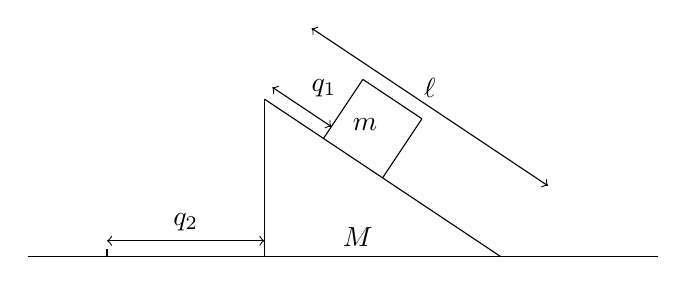
\begin{tikzpicture}
   % X axis
   \draw (-4,-0) -- (4,-0);
   \draw (-3,-0) -- (-3,0.1);
   % Wedge
   \draw (-1,0) -- (-1,2);
   \draw (-1,2) -- (2,0);
   \draw (-1,0) -- node[above left]{$M$} (2,0);
   \draw[<->] (-0.4,2.9) -- node[above]{$\ell$} (2.6,0.9);
   \draw[<->] (-3,0.2) -- node[above]{$q_2$} (-1,0.2);
   % Block
   \draw (-0.25,1.5) -- node[below right]{$m$} (0.25,2.25);
   \draw (0.25,2.25) -- (1,1.75);
   \draw (0.5,1) -- (1,1.75);
   \draw[<->] (-0.9,2.15) -- node[above right]{$q_1$} (-0.15,1.65);
  \end{tikzpicture}
 \end{center}
 \item A system of three masses is arranged on the corners of a foldable frame with length $a$ (\textit{i.e.} the mass $m_2$ can move along the vertical axis as $\theta$ changes).  The whole system is rotating about the vertical axis with angle $\phi$.  Determine the Lagrangian as a function of $\phi$ and $\theta$.  From the equations of motion determine the equilibrium angle for given $\dot\phi = \omega$.
 \begin{center}
  \begin{tikzpicture}
   % Axis
   \draw (0,-3) -- (0,3);
   % Frame
   \draw (0,+2.5) -- node[above right]{$a$} (+2,0) node[right]{$m_1$};
   \draw (0,+2.5) -- node[above left]{$a$} (-2,0) node[left]{$m_1$};
   \draw (+2,0) -- node[below right]{$a$} (0,-2.5) node[below left]{$m_2$};
   \draw (-2,0) -- node[below left]{$a$} (0,-2.5);
   % Angle
   \draw (0,1.5) node[below right]{$\theta$} arc (-90:-51:1);
  \end{tikzpicture}
 \end{center}
\end{enumerate}

\end{document}
